\documentclass[a4paper,twoside,openany]{book} 

%% Using the Custom Style File
\usepackage{ManningBook}
%\usepackage{showframe}
\usepackage{kantlipsum}

\setlength{\textheight}{665pt}
\setlength{\footskip}{40pt}

\allowdisplaybreaks

\begin{document}
	
	%% Cover, Title Page, TOC, Preface, and others
	\frontmatter
	
	% The Cover
	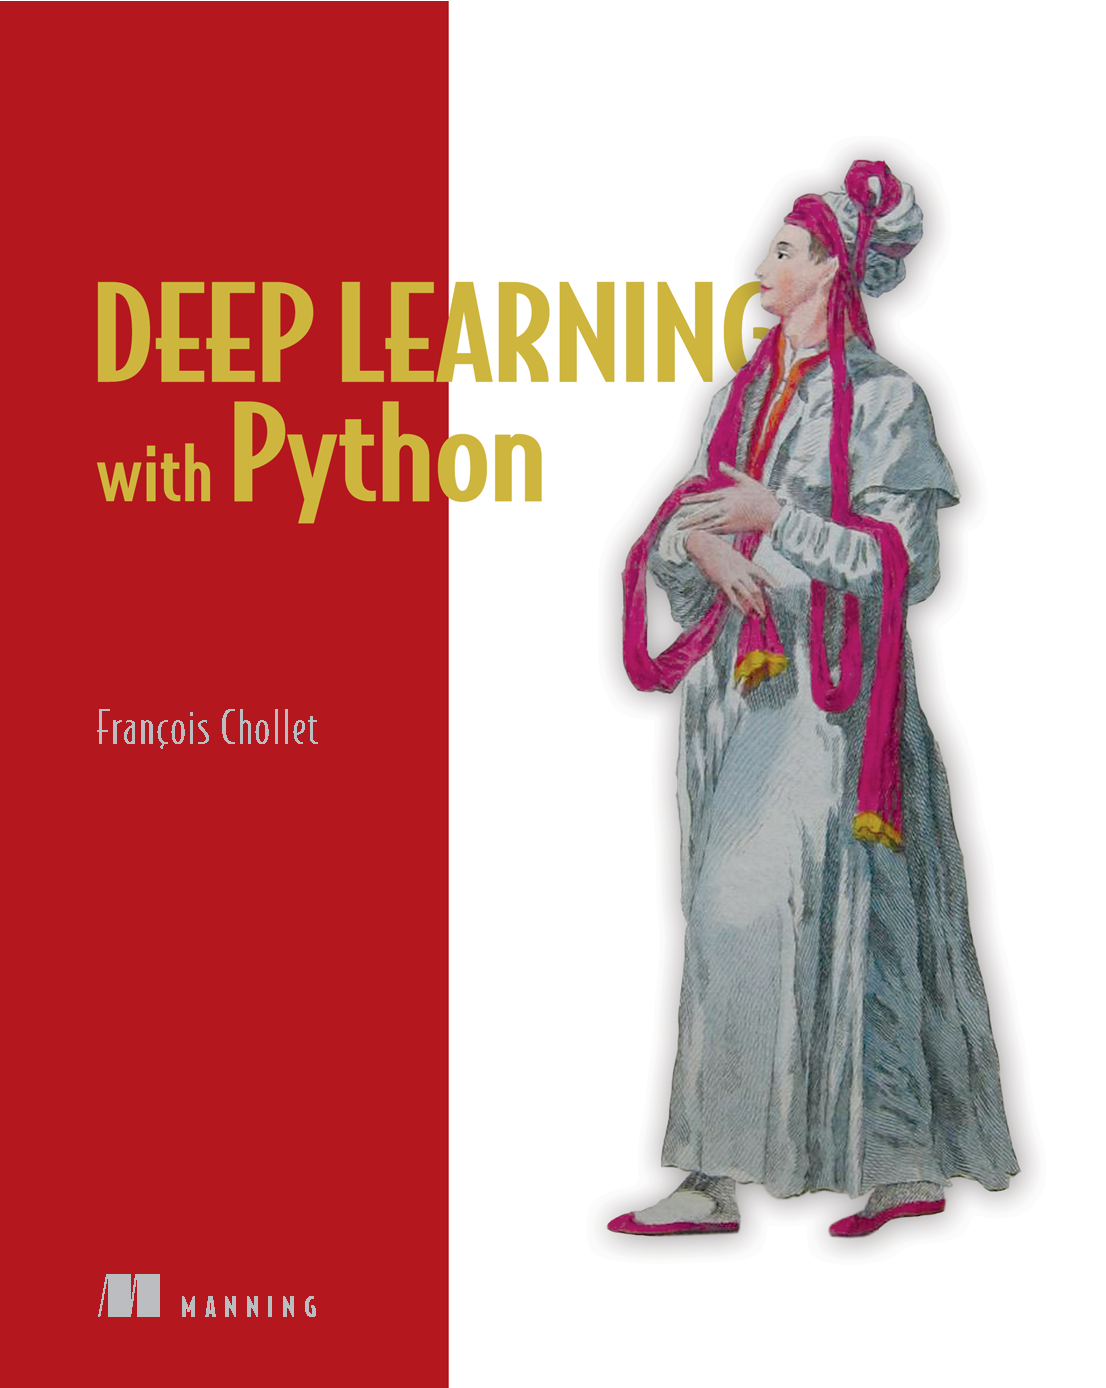
\includepdf[width=\paperwidth, height=\paperheight]{
		External PDF Pages/DLCover.pdf}
		
	% The Book Title Standalone Page and Consecutive Blank One
	\thispagestyle{empty}
	\centerline{\HeaderFont\fontsize{16}{18}\color{ChapTitleColor}\selectfont 
		Deep Learning with Python}
	\afterpage{\blankpage}
	
	\pagebreak
	
	% The Book Title + Author Name + Publisher Page
	\let\cleardoublepage\clearpage
	\thispagestyle{empty}
	\vspace*{7cm}
	{\ChapHeadFont\fontsize{50}{52}\color{ChapTitleColor} 													\selectfont \raggedleft Deep Learning \\[8pt] \hspace{6.5cm} with Python}
	
	\vspace{3cm}
	
	{\hfill \AuthorNameFont\fontsize{14}{16}\selectfont 
			FRAN\MakeUppercase{ç}OIS CHOLLET}
	%% Branding
	\begin{figure}[b]
		\hfill\includesvg[scale=0.3]{manning_logo.svg} \tikzmark{ManningBrand}
	\end{figure}
	\begin{tikzpicture}[remember picture, overlay]
		\node[anchor=north] at ([shift={(-1.4,0)}]{pic cs:ManningBrand}) 											{\HighlightBodyFont\fontsize{18}{20}\selectfont MANNING};
		\node[anchor=north] at ([shift={(-1.85,-0.7)}]{pic cs:ManningBrand}) 										{\HighlightBodyFont\fontsize{14}{16}\selectfont SHELTER ISLAND};
	\end{tikzpicture}
	
	\newpage
	
	\thispagestyle{empty}
	
	{
	\AuthorNameFont\fontsize{11}{12}\selectfont
	\noindent For online information and ordering Of this and other Manning books, please visit \\[2pt]
	www.manning.com. The publisher offers discounts on this book when ordered in quantity. \\[2pt] 
	For more information, please contact
	
	\begin{verse}
		Special Sales Department \\[1pt]
		Manning Publications Co. \\[1pt]
		20 Baldwin Road \\[1pt]
		PO Box 761 \\[1pt]
		Shelter Island, NY 11964 \\[1pt]
		Email: orders@manning.com
	\end{verse}
	
	\vspace{0.5cm}
	
	\noindent\textcopyright\ 2018 by Manning Publications Co. All rights reserved.
	
	\vspace{30pt}
	
	\par\noindent No part Of this publication may be reproduced, stored in a retrieval system, or 			transmitted, in any form or by means electronic, mechanical, photocopying, or otherwise, without 		prior written permission of the publisher.
	
	\vspace{30pt}
	
	\par\noindent Many Of the designations used by manufacturers and sellers to distinguish their 			products are clairned as tradernarks. those designations appear in the book, and Manning 				Publications was aware of a trademark claim, the designations have been printed in initial caps or 		all caps.
	
	\vspace{30pt}
	
	\llap{\scalebox{0.8}{$\acidfree$}\hspace{4pt}\vspace*{-11pt}}\noindent Recognizing the importance 		of preserving what has been written, it is Manning's policy to have the books we publish printed on 	acid-free paper, and we exert our best efforts to that end. Recognizing also our responsibility to 		conserve the resources of our planet, Manning books are printed on paper that is at least 15 			percent recycled and processed without the use of elemental chlorine.
	
	\vspace{1.5cm}
	
	\noindent \includesvg[scale=0.25]{manning_logo.svg} \tikzmark{ManningLower}
	
	\begin{tikzpicture}[remember picture, overlay]
		\node[anchor=west] at ([shift={(0,0.65)}]{pic cs:ManningLower}) {Manning Publications Co.};
		\node[anchor=west] at ([shift={(0,0.25)}]{pic cs:ManningLower}) {20 Baldwin Road};
		\node[anchor=west] at ([shift={(0,-0.20)}]{pic cs:ManningLower}){PO Box 761};
		\node[anchor=west] at ([shift={(0,-0.60)}]{pic cs:ManningLower}){Shelter Island, NY 11964};
		\node[anchor=west] at ([shift={(5,-1.3)}]{pic cs:ManningLower}){ 
		\setlength\extrarowheight{-7pt}
		\begin{tabular}{r@{\hspace{7pt}}l}
			Development editor:           & Toni Arritola               \\
			Technical development editor: & Jerry Gaines                \\
			Review editor:            & Aleksandar Dragosavljevi$\acute{\text{c}}$\\
			Project editor: 			  & Tiffany Taylor              \\
			Copyeditor: 				  & Tiffany Taylor              \\
			Proofreader: 				  & Katie Tennant               \\
			Technical proofreaders: 	  & Alex Ott and Richard Tobias \\
			Typesetter: 				  & Dottie Marsico              \\
			Cover designer: 			  & Marija Tudor
		\end{tabular}
		};
	\end{tikzpicture}
	
	\vspace{4cm}
	
	\begin{verse}
		ISBN 9781617294433 \\[3pt]
		Printed in the United States of America \\[3pt]
		1 2 3 4 5 6 7 8 9 10 - EBM - 22 21 20 19 18 17
	\end{verse}
	
	}
	
	%% The Short TOC
	\renewcommand{\contentsname}{brief contents}
	\setcounter{tocdepth}{0} 
	\tableofcontents 
	\thispagestyle{FMPageStyle}
	
	\afterpage{
		\null
		\thispagestyle{empty}
	}
	
	\thispagestyle{FMPageStyle}	
	\newpage
	
	\pagestyle{FrontMatterMainPages} %%% Style for Consecutive Pages
		
	\chapter*{preface} \chaptermark{preface}
	\thispagestyle{FMPageStyle}	
	\kant[1-6]
	
	\chapter*{acknowledgments} \chaptermark{acknowledgments}
	\thispagestyle{FMPageStyle}	
	\kant[1]
	
	\chapter*{about this book} \chaptermark{about this book}
	\thispagestyle{FMPageStyle}	
	\kant[1-6]
	
	\chapter*{about the author} \chaptermark{about the author}
	\thispagestyle{FMPageStyle}	
	\begin{wrapfigure}{l}{0.3\textwidth}
		\centering
		\vspace{-\baselineskip} % Aligns the Upper Tip of Image to 1st Line
		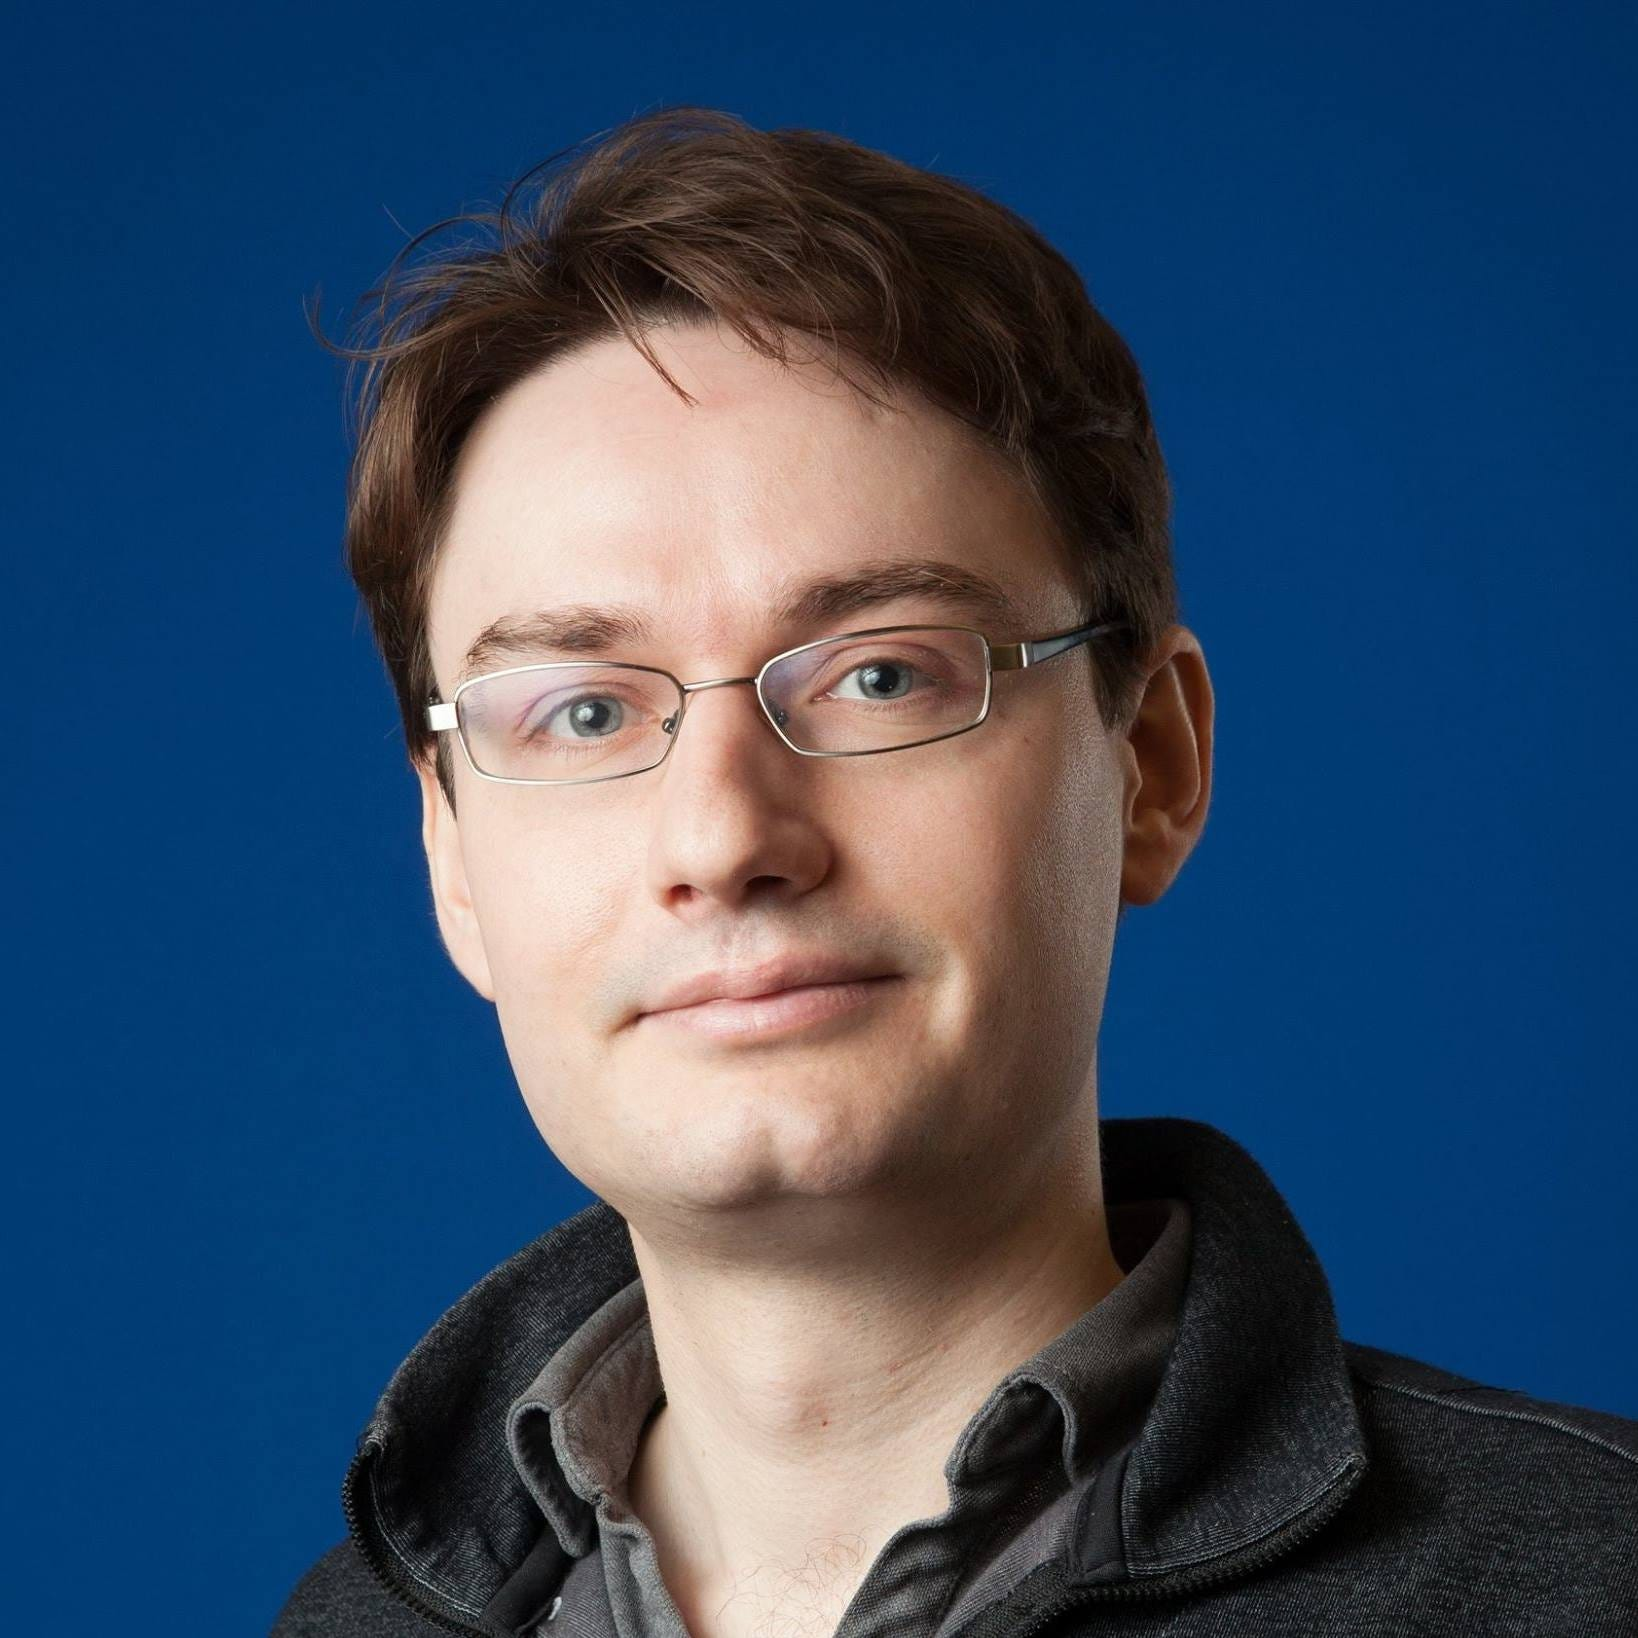
\includegraphics[width=\linewidth]{author.jpg}
	\end{wrapfigure}
	\kant[1]
	
	\chapter*{about the cover} \chaptermark{about the cover}
	\thispagestyle{FMPageStyle}	
	\kant[1]
	
	\afterpage{\blankpage}
	
	%%%%%%%%%%%%%%%%%%%%%%%%%%%%%%%%%%%%%%%%%%%%%%%%%%%%%%%%%%%%%%%%%%%%%%%%%%
	%%%%%%%%%%%%%%%%%%%%%%%%%%%%%%%%%%%%%%%%%%%%%%%%%%%%%%%%%%%%%%%%%%%%%%%%%%
	
	%% Main Content 
	\mainmatter
	
	\part[FUNDAMENTALS OF DEEP LEARNING]{Fundamentals \\ of deep learning}	
	\thispagestyle{empty}
	
	\begin{spacing}{1.3}
	\BigPartLetter{C}hapters 1-4 of this book will give you a foundational 									understanding of what deep learning is, what it can achieve, and how it works. It will also make 		you familiar with the canonical workflow for solving data problems using deep learning. If you 
	aren 't already highly knowledgeable about deep learning, you should definitely begin by reading 		part I in full before moving on to the practical applications in part 2.
	\end{spacing} \index{Artificial Neural Networks}
	
	\afterpage{
		\null \thispagestyle{empty} \newpage	
	}
	
	\chapter[Vectors, matrices, and tensors in machine learning]{Vectors, matrices, and \\ tensors in 		machine learning}
	
	\pagestyle{ChapterMainStyle} %% Applying the Main Style
	
	\begin{ChapterTopics}{0.7}
		\item Vectors and matrices and their role in data science
		\item Working with eigenvalues and eigenvectors
		\item Finding the axes of a hyper-ellipse
	\end{ChapterTopics} \index{Convolutional Neural Networks}
	
	\begin{spacing}{1.5}
		\section{First Section}
		\kant[1]
		\begin{ManNote}
			The dot product notation can compactly represent the model output as 
			$y = \overrightarrow{w}\cdot\overrightarrow{x}+b$.  The representation 									does not increase in size even when the number of inputs and weights is large.
		\end{ManNote} \index{Recurrent Neural Networks}
		\kant[1]
		
		\subsection{First Subsection}
		\kant[1] \index{Deep Learning Frameworks}
		
		\begin{ManHighlight}{Linear Algebra Essentials}
			\par\noindent In linear algebra, vectors, matrices, and tensors form the 								cornerstone of understanding various mathematical concepts and real-world applications. 				Vectors represent quantities with both magnitude and direction, while matrices serve as 				arrays of numbers facilitating operations like addition, multiplication, and 							transformations. Tensors extend these concepts, enabling the representation of higher-order 			data structures. Mastery of these fundamental objects is essential for tackling complex 				problems across numerous fields, from physics to machine learning.
		\end{ManHighlight} \index{Supervised Learning}
		
		\kant[1]
		
		%% Code Listing and Annotation
		% 1. List and Throw TiKZ Marks
		\begin{lstlisting}[caption= Introducting Matrices via PyTorch]
			@\\[30pt]@
			X@\tikzmark{XMatrix1}@ = torch.tensor( @\tikzmark{XTensor}@
					[
								[0.11, 0.09], [0.01, 0.02], [0.98, 0.91],
								[0.12, 0.21], [0.98, 0.99], [0.85, 0.87],
								[0.03, 0.14], [0.55, 0.45] @\tikzmark{XMatrix2}@
					]
			)
			
			print(''Shape of the matrix is: ''.format(X.shape)) @\tikzmark{XShape}@
			
			first_element = X[0, 0] @\tikzmark{XFirst}@
			
			row_0 = X[0, :]     @\tikzmark{XRow0}@
			row_1 = X[1, 0:2]   @\tikzmark{XRow1}@
			
			column_0 = X[:, 0]  @\tikzmark{XCol0}@
			column_1 = X[:, 1]  @\tikzmark{XCol1}@
		\end{lstlisting}
		% 2. Annotate at Placed Marks: <Run Multiple Times to Resolve !!>
		\begin{tikzpicture}[remember picture, overlay,
							every node/.append style={font=\HighlightTitleFont}]
			%% Annotation 1
			\RightArrowedCornerNote{Ann1}{-0.5cm}{-1pt}{XMatrix1}{~A matrix is a 2D 								array of numbers: i.e., a 2D tensor. \\[-5pt] ~The entire training data input set for a 				machine-learning model can be viewed as a matrix. \\[-5pt] ~Each input instance is one 					row. \\[-5pt] ~Row count $\equiv$ number of training examples, column count $\equiv$ 					training instance size}{-1}{2}{-0.4}{0.2}
			%% Annotation 2
			\RightWalledNote{Ann2}{4cm}{0.65cm}{XMatrix2}{~Cat-brain training data 									input: \\[-5pt]~8 examples, each with two \\[-5pt] ~values (hardness, sharpness). \\[-5pt] 				~An 8 x 2 tensor is created by \\[-5pt] ~directly specifying values.}{-0.5}{1.1}{1.1}
			%% Annotation 3
			\RightWalledNote{Ann3}{0.8cm}{3pt}{XShape}{~The shape of a tensor is a 									list. \\[-5pt] ~For a matrix, the first list \\[-5pt] ~element is num rows; the \\[-5pt] 				~second list element is num \\[-5pt]~columns.}{-0.8}{1.1}{1.1}
			%% Annotation 4
			\RightWalledNote{Ann4}{1.5cm}{3pt}{XFirst}{~Square brackets extract \\[-5pt]~individual 				matrix elements.}{-1}{0.4}{0.4}
			%% Annotations 5-8
    		\LeftArrowedNote{Ann5}{1.5cm}{3pt}{XRow0}{~A standalone colon operator denotes all possibel 			indices.}{-1.6}
    		\LeftArrowedNote{Ann6}{1.5cm}{3pt}{XRow1}{~The colon operator denotes the range of 						indices.}{-1.3}
    		\LeftArrowedNote{Ann7}{1.5cm}{3pt}{XCol0}{~0th column}{-1}
    		\LeftArrowedNote{Ann8}{1.5cm}{3pt}{XCol1}{~1st column}{-1}
		\end{tikzpicture}
		
		\kant[1] \index{Unsupervised Learning}
		
		\begin{figure}[h]
			\centering
			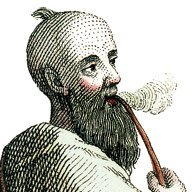
\includegraphics[scale=0.7]{Manning.jpg}
			\caption{\centering Some Temporary Caption Text}
		\end{figure}				
		
		\vspace{0.5cm}
		
		\ManHeadLine{15}{16}{RECENTLY ADDED MANNING TITLES \\[-8pt]} 
		
		\begin{figure}[h]
    		\centering 
		    \begin{subfigure}[b]{0.3\textwidth}
		        \centering
		        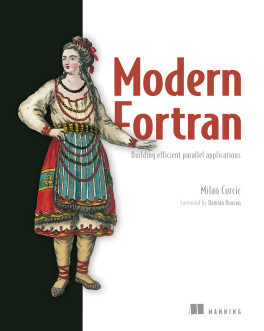
\includegraphics[width=0.45\textwidth]{Curcic-MF-HI.png}
		        \caption{\centering Modern Fortran}
		    \end{subfigure}
		    %
		    \begin{subfigure}[b]{0.3\textwidth}
		        \centering
		        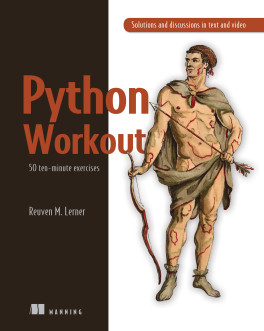
\includegraphics[width=0.45\textwidth]{Lerner-Python-HI.png}
		        \caption{\centering Python Workout}
		    \end{subfigure}
		    \\[10pt]
		    \begin{subfigure}[b]{0.3\textwidth}
		        \centering
		        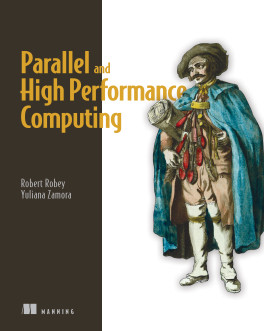
\includegraphics[width=0.45\textwidth]{Robey-PHPC-HI.png}
		        \caption{\centering Parallel Computing}
		    \end{subfigure}
		    %
		    \begin{subfigure}[b]{0.3\textwidth}
		        \centering
		        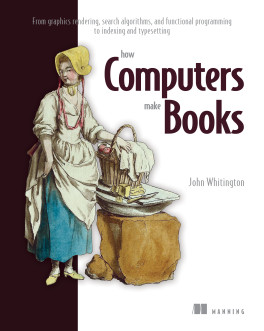
\includegraphics[width=0.45\textwidth]{Whitington-HI.png}
		        \caption{\centering Computers and Books}
		    \end{subfigure}
		    \caption{\centering Some Recent Manning Books}
		\end{figure}		
		
		\kant[1-2] \index{Reinforcement Learning}
		
		\vspace{0.5cm}
		
		\ManHeadLine{15}{16}{SIDEWAY CAPTIONING FOR FLOATS \\[-8pt]}
		
		%% Sideway Captioning for Floats: 							
		% 1. Using the sidecap Package with <rightcaption> global option
		{
			\sidecaptionvpos{figure}{t} % Vertical Positioning of Caption also <c,b>
			\begin{SCfigure}[10][h]
			  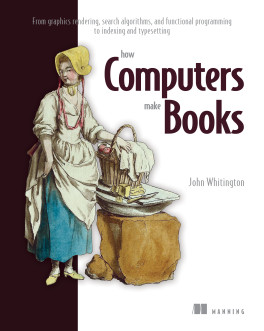
\includegraphics[width=0.4\textwidth]{Whitington-HI.png}
			  \caption{How Computers Make Books introduces what’s wonderful about computer science by 					showing how computers have transformed art of publishing books. Author and publishing 					software developer John Whitington reveals the elegant computer science solutions 						invented to solve big publishing challenges.
			  	}
			\end{SCfigure}
		} \index{Gradient Descent}
		% 2. Using minipage environment
		\begin{figure}[h]
			\begin{minipage}{0.5\textwidth}
				\caption{How Computers Make Books introduces what’s 													wonderful about computer science by showing how computers have transformed art of 						publishing books. Author and publishing software developer John Whitington reveals 						the elegant computer science solutions invented to solve big publishing challenges.}
			\end{minipage} \index{Backpropagation}
			\hspace{10pt}
			\begin{minipage}{0.5\textwidth}
				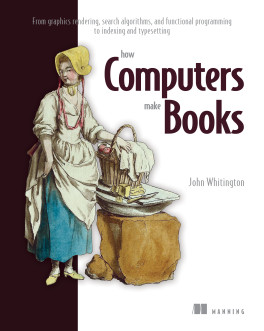
\includegraphics[width=0.5\textwidth]{Whitington-HI.png}
			\end{minipage} \index{Activation Functions}
		\end{figure}
		
		\kant[1] \index{Dropout Regularization}
		
		\vspace{0.25cm}
		
		\begin{table}[h]
	    	\caption{Example training dataset for our toy machine 
	    		learning-based cat brain}
	    	\centering
		    \begin{tblr}{
			        colspec={|c|c|c|c|},
			        row{1}={bg=TableHeadRowColor},
			        rowsep=5pt
			    }
		        \hline
		        & Input Value: Hardness & Input Value: Sharpness & 
		        	Output: Threat Score \\
		        \hline
		        0 & 0.11 & 0.09 & -0.8  \\
		        1 & 0.01 & 0.02 & -0.97 \\
		        2 & 0.98 & 0.91 & 0.89  \\
		        3 & 0.12 & 0.21 & -0.68 \\
		        4 & 0.98 & 0.99 & 0.95  \\
		        5 & 0.85 & 0.87 & 0.74  \\
		        6 & 0.03 & 0.14 & -0.88 \\
		        7 & 0.55 & 0.45 & 0.00  \\
		        \hline
	    	\end{tblr}
		\end{table} \index{Batch Normalization}
		
		\kant[1]
		
		\begin{align}
		  \begin{aligned}
		    a_0 + \cfrac{1}{
		      a_1 + \cfrac{1}{
		        a_2 + \cfrac{1}{
		          a_3 + \cdots}}}
		  \end{aligned}
		  \label{equation:one}
		\end{align}
		
		\begin{align}
		  \begin{aligned}
		    c_0 &= \cfrac{3}{1} = 3.0 \\
		    c_1 &= 3 + \cfrac{1}{7} = \frac{22}{7} = 3.142857142857143 \\
		    c_2 &= 3 + \cfrac{1}{7 + \cfrac{1}{15}} = \frac{333}{106} = 3.141509433962264 \\
		    c_3 &= 3 + \cfrac{1}{7 + \cfrac{1}{15 + \cfrac{1}{1}}} = \frac{355}{113} 
		    	= 3.1415929203539825 \\
		    c_4 &= 3 + \cfrac{1}{7 + \cfrac{1}{15 + \cfrac{1}{1 + \cfrac{1}{292}}}} =
		  \frac{103993}{33102} = 3.1415926530119025 \\
		  \end{aligned}
		  \label{equation:two}
		\end{align}
		
		{
		\fontsize{10}{0}\selectfont
		\begin{align}
		  \begin{aligned}
		    \frac{44237}{111361} =
		      0 + \cfrac{1}{
		        2 + \cfrac{1}{
		          1 + \cfrac{1}{
		            1 + \cfrac{1}{
		              13 + \cfrac{1}{
		                1 + \cfrac{1}{
		                  8 + \cfrac{1}{
		                    6 + \cfrac{1}{
		                      1 + \cfrac{1}{
		                        2 + \cfrac{1}{
		                          1 + \cfrac{1}{
		                            1 + \cfrac{1}{
		                  3}}}}}}}}}}}} = [0; 2, 1, 1, 13, 1, 8, 6, 1, 2, 1, 1, 3]
		  \end{aligned}
		  \label{equation:three}
		\end{align}
		}
		
		\kant[1-2]
		
		\begin{ChapterSummary}
			\item Understanding the fundamental concepts of vectors, matrices, and tensors 
			in linear algebra.
			\item Exploring the geometric and algebraic representations of vectors and their 
			basic operations.
			\item Investigating matrices as arrays of numbers and their operations, including addition, 			multiplication, and special matrix types.
			\item Analyzing linear transformations and their connection to matrices, 								eigenvalues, and eigenvectors.
			\item Introducing tensors as generalizations of vectors and matrices, with applications in 				various fields such as physics, engineering, and machine learning.
		\end{ChapterSummary} \index{Transfer Learning}
	\end{spacing}	
	
	\pagebreak
	
	\chapter{What is deep learning?} \index{Generative Adversarial Networks}
	\section{Artificial intelligence, machine learning, and deep learning}	
		\subsection{Aniftcial intelligence}
		\subsection{Machine learning} \index{Autoencoders}
		\subsection{Learning representations from data} 
			\index{Natural Language Processing}
		\subsection{Understanding how deep learning works} 
			\index{Image Classification}
		\subsection{What deep learning has achieved so far} \index{Object Detection}
		\subsection{Don 't believe the short-term hype} 
			\index{Semantic Segmentation}
	\section{Before deep learning: a brief history of machine learning}
		\subsection{Probabilistic modeling} \index{Speech Recognition}
		\subsection{Early neural networks} \index{Time Series Prediction}
		\subsection{Kema methods} \index{Hyperparameter Tuning}
		\subsection{Decision trees, random forests, and gradient boosting machines}
		\subsection{Back to neural networks} \index{Model Evaluation Metrics}
		\subsection{What makes deep learning different}
			\index{Overfitting}
			\index{Underfitting}			

	\chapter{Orthogonality and Independence in Linear Algebra}
		\index{Data Augmentation}
	\chapter{Algorithms of Reinforcement Learning for Robotics}
		\index{Fine-tuning}
	
	%%%%%%%%%% SECOND PART %%%%%%%%%%%%%%
	\part[DEEP LEARNINF IN PRACTICE]{Deep learning \\ in practice}	
	\thispagestyle{empty}
	
	\begin{spacing}{1.3}
	\BigPartLetter{C}hapters 4-8 of this book will give you a foundational 									understanding of what deep learning is, what it can achieve, and how it works. It will also make 		you familiar with the canonical workflow for solving data problems using deep learning. If you 
	aren 't already highly knowledgeable about deep learning, you should definitely begin by reading 		part I in full before moving on to the practical applications in part 2.
	\end{spacing} \index{Long Short-Term Memory (LSTM)}
	
	\afterpage{
		\null \thispagestyle{empty} \newpage	
	}
	
	\chapter{Fundamentals of machine learning}
		\index{Attention Mechanism} \index{Algorithmic Complexity}
		\index{Bayesian Inference} \index{Clustering Techniques}
		\index{Dimensionality Reduction} \index{Ensemble Methods}
		\index{X-means Clustering} \index{Yield Curve Prediction}
		\index{Decision Boundary} \index{Evolutionary Algorithms}
		\index{Adversarial Examples} \index{Batch Gradient Descent}
		\index{Capsule Networks} \index{Deep Reinforcement Learning}
		\index{Ensemble Learning} \index{Fuzzy Logic}
	\chapter{Generative deep learning}
		\index{Explainable AI (XAI)} \index{Feature Engineering}
		\index{Graph Neural Networks} \index{Hierarchical Clustering}
		\index{Instance-based Learning} \index{Kernel Methods}
		\index{Zero-shot Learning} \index{Active Learning}
		\index{Genetic Algorithms} \index{Hebbian Learning}
		\index{Instance Segmentation} \index{Knowledge Graphs}
		\index{Label Smoothing} \index{Memory Augmented Networks}
		\index{Non-Maximum Suppression} \index{One-shot Learning}
	\chapter{Advanced deep-learning best practices}
		\index{Self-Supervised Learning} \index{Latent Dirichlet Allocation}
		\index{Model Interpretability} \index{Neural Architecture Search}
		\index{Online Learning} \index{Precision-Recall Curve}
		\index{Bayesian Optimization} \index{Collaborative Filtering}
		\index{Policy Gradient Methods} \index{Quantum Computing}
		\index{Random Forests} \index{Self-Organizing Maps}
		\index{Text Mining} \index{Unstructured Data} 
		\index{Variational Autoencoders} \index{Weight Initialization}
		\index{Temporal Convolutional Networks} \index{Value Iteration}
		\index{Universal Approximation Theorem} \index{Value Iteration}
		\index{Weak Supervision} \index{XGBoost} \index{Yield Curve Modeling}
		\index{Zero-day Attacks Detection} \index{Attention-based Models}
		\index{Bayesian Deep Learning} \index{Contrastive Learning}
		\index{Dropout Layers} \index{Explainability in AI}
	\chapter{Deep learning for computer vision}
		\index{Federated Learning} \index{Quantum Machine Learning}
		\index{Regularization Techniques} \index{Stochastic Gradient Descent}

	%%%%%%%%%%%%%%%%%%%%%%%%%%%%%%%%%%%%%%%%%%%%%%%%%%%%%%%%%%%%%%%%%%%%%%%%%%
	%%%%%%%%%%%%%%%%%%%%%%%%%%%%%%%%%%%%%%%%%%%%%%%%%%%%%%%%%%%%%%%%%%%%%%%%%%
	
	%% Appendix, Bibliography, Index, and others

	\appendix 
	
	% Necessary Step to Proceed with Appendix Chapters made with \chapter*{} 
	\setcounter{chapter}{1} 
	% Redefining \chapter*{} format for Appendices
	\titleformat{name=\chapter,numberless}[display]
 	{\vspace*{4cm}\raggedleft 
 	 \ChapHeadFont\fontsize{30pt}{30pt}\selectfont\color{ChapTitleColor}}
  	{appendix \thechapter} 
  	{10pt}{}[\LowerRule{0.7}]
  	
  	%% Applying the Appendix Page Header
  	\pagestyle{AppendixChapStyle}
	
	% We use \chapter*{} instead of normal conuted one in order to ommit the Appendix chapters from the 	"brief contents".
	\chapter*{Installing Keras and its \\ dependencies on Ubuntu} 
		\chaptermark{Installing Keras and its dependencies on Ubuntu}
	\kant[1-4]
	\section{Installing the Python scientific suite}
	\kant[1-6]
	
	\stepcounter{chapter} 
	\chapter*{Running JuPyter notebooks \\ on an EC2 GPU instance} 
		\chaptermark{Running JuPyter notebooks on an EC2 GPU instance}
	\kant[1-4]
	\section{Setting up an AWS GPU instance}
	\kant[1-6]
	
	%%%%%%%%%%%%%%%%%%%%%%%%%%%%%%%%%%%%%%%%%%%%%%%%%%%%%%%%%%%%%%%%%%%%%%%%%%
	%%%%%%%%%%%%%%%%%%%%%%%%%%%%%%%%%%%%%%%%%%%%%%%%%%%%%%%%%%%%%%%%%%%%%%%%%%
	
	\backmatter 
	
	% Redefining \chapter*{} format for the Index both the <title> option to the \makeindex[] in the 		preamble and the \titleformat commands control the numberless appearance of the "index" title 			head. I chose to empty the latter, and leave the styling in the \makeindex[]
	\titleformat{name=\chapter,numberless}[display]{}{}{0pt}{}
	
	% Applying the Index Page Style
	\pagestyle{IndexPagesStyle}
	
	%% The Index
	\printindex

\end{document}
